\subsection{\yytwotau channel}{\Large\bfseries}
\label{sec:yy2taus}

This section describes.......

\subsubsection{Event selection}

Events are selected for this channel if there are at least two photons and at least two oppositely charged \tauh, which satisfy the criteria outlined in Section~\ref{sec:}. The diphoton invariant mass is initially required to fall within a broad mass window of 105 GeV < $m_{\gamma\gamma}$ < 160 GeV. In order to remain orthogonal to the ATLAS search for $HH \rightarrow \gamma\gamma$$b\overline{b}$ [\ref{ref:}], any event with b-jet using the 70\% efficient working point is rejected.

\subsubsection{Background composition}

This analysis is affected both by backgrounds from single-Higgs-boson production and by non-resonant backgrounds with continuum \myy spectra. The major single Higgs boson production contributing to the background are associated production with a Z boson ($ZH$), associated production with a top quark pair (\ttH). As for continuum backgrouds, the major contributions are vector boson production associated with photons (\Vyy) and multi-jet processes associated with photons (\yyjet).

Simulated samples are used to model single-Higgs-production and vector boson production associated with photons (\Vyy), while processes with fake-\tauh are estimated using data-driven techniques, as discussed below. In \yytwotau channel, the fake-\tauh backgrounds are from multi-jet processes in the sense that some of QCD jets can be mis-identified as hadronically decay $\tau$ jets. A data-driven fake-factor method is used to estimate the multi-jet processes as decribed in Section \ref{sec:}.

Events with electrons and muons that are misidentified as \tauh objets, dominantly coming from the \Vyy production ($V \rightarrow l^+l^-$), represent a minor background in the analysis and they are estimated from simulation.

\subsubsection{\yyjet with fake-\tauh in the \yytwotau channel}

To estimate the \yyjet background contribution we employ a fake factor method. This method is schematically depicted in Fig.\ref{fig:yy2tau:FFschem}.
\begin{figure}[]
	\begin{center}
	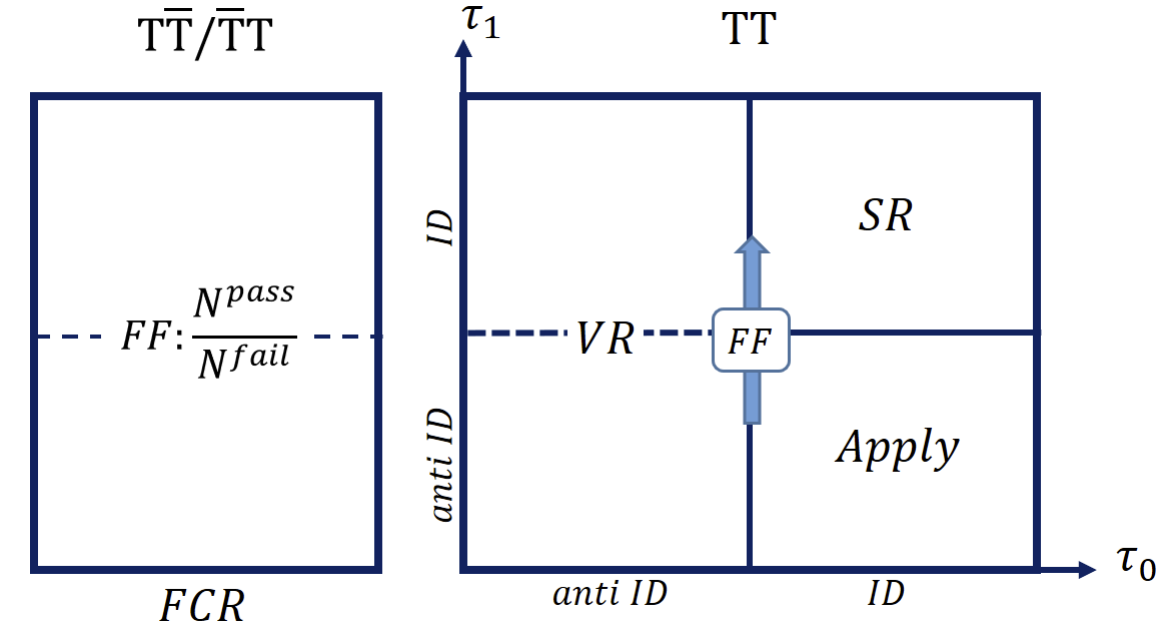
\includegraphics[width=0.65\textwidth]{figures/yy2tau/FFschem.png}
	\caption{\label{fig:yy2tau:FFschem} schematic depiction of the application of the fake factor mehthod used to estimate the \yyjet background in the di-Higgs \yytwotau channel. Left: Fake factors are calculated in the $FCR$ with tight/anit-tight ($T\overline{T}$/$\overline{T}T$) identification on the two photons candidates. Right: Fake factors are then applied to the "Apply" region with two tight photons, loose leading \tauh and anti-loose subleading \tauh to estimate \yytwotau contribution in signal region (SR). A validation region (VR) is also defined as event with two tight photons and anti-loose leading \tauh. }
	\end{center}
\end{figure}

A fake-\tauh control region ($FCR$) is designed to derive the fake factors with the same definition as the signal region, except that the tight photon-ID requirement on one of the two photon candidates is inverted ($T\overline{T}$/$\overline{T}T$). To have as large statistic as possible, no tau-ID requirement is applied to the leading \tauh candidate and no oppositely-charged requirement is applied to the two \tauh candidates. The tau-ID fake factors, $f_{\tau_{1}-ID}$, are then defined as the number of events with two \tauh candidates passing loose tau-ID, divided by the number of events with leading \tauh candidate passing loose tau-ID while sub-leading \tauh candidate failing loose tau-ID.
\begin{equation}
f_{\tau_{1}-ID}({p_{T}}_{\tau_{1}},N_{trks})=\frac{N^{pass\;\tau_{1}-ID,\;FCR}_{data}({p_{T}}_{\tau_{1}},N_{trks}) - N^{pass\;\tau_{1}-ID,\;FCR}_{other\;MCs}({p_{T}}_{\tau_{1}},N_{trks})}{N^{fail\;\tau_{1}-ID,\;FCR}_{data}({p_{T}}_{\tau_{1}},N_{trks}) - N^{fail\;\tau_{1}-ID,\;FCR}_{other\;MCs}({p_{T}}_{\tau_{1}},N_{trks})}
\end{equation}
where $\tau_{1}$ denotes the subleading \tauh candidate and $N_{trks}$ is the number of associated tracks of the subleading \tauh candidate. The tau-ID fake factors are determined as a function of transverse momentum of subleading \tauh and measured separately depending on the number of associated tracks of the subleading \tauh candidate. All other significant backgrounds () are subtracted in fake-\tauh control region before computing the fake factors to give a very pure multi-jets region and avoid possible biased due to differences in normalization and shape of the other backgrounds between the individual regions.


The $FF$s are applied to a control region with the same definition as the signal region, except that the loose tau-ID requirement on the subleading \tauh candidate is inverted (fail-ID region). This gives both the shape and normalization of the \yyjet contribution. The \yyjet contribution in the signal region, $N_{\yyjet}$ is then predicted by weighting the events from the fail-ID region by their fake factors:
\begin{equation}
N_{\yyjet}({p_{T}}_{\tau_{1}},N_{trks})=f_{\tau_{1}-ID}({p_{T}}_{\tau_{1}},N_{trks})\times(N^{fail\;\tau_{1}-ID}_{data}({p_{T}}_{\tau_{1}},N_{trks}) - N^{fail\;\tau_{1}-ID}_{other\;MCs}({p_{T}}_{\tau_{1}},N_{trks}))
\end{equation}
Again, all other significant backgrounds are subtracted in fail-ID region before applying the fake factors. 

The subleading \tauh candidate $p_{T}$ distributions in the $FCR$ are shown in Fig.\ref{fig:yy2tau:FCRs}, separately for 1- and 3-prong \tauh. The measured fake factors are shown in Fig.\ref{fig:yy2tau:FFs} and only statistical uncertainty is ploted. A closure test is performed to show that the derived fake factors can yield distribution consistent with data with regard to other observables by applying the fake factor back to the FCR, As shown in Fig.\ref{fig:yy2tau:Closure}.

To validate the fake factor method, a validation region should be as close as possible to the signal region, meanwhile, should be better have adequate statistic. A first thought is to do the validation in the sideband, [105, 120]\&[130, 160]GeV, of \myy distribution (signal region is [120, 130]GeV), which fails the statistic requirement. Therefore, the validaton region is finally defined requiring events containing two tight photons and two oppositely charged \tauh candidates, among which the leading \tauh candidate fails loose tau-ID. As shown in Fig.\ref{fig:yy2tau:VRs}, the fake factor method estimation is compared to observed data in VR with regard to \myy. more validation plots to be added for MVA input variables...

\begin{figure}
	\centering
	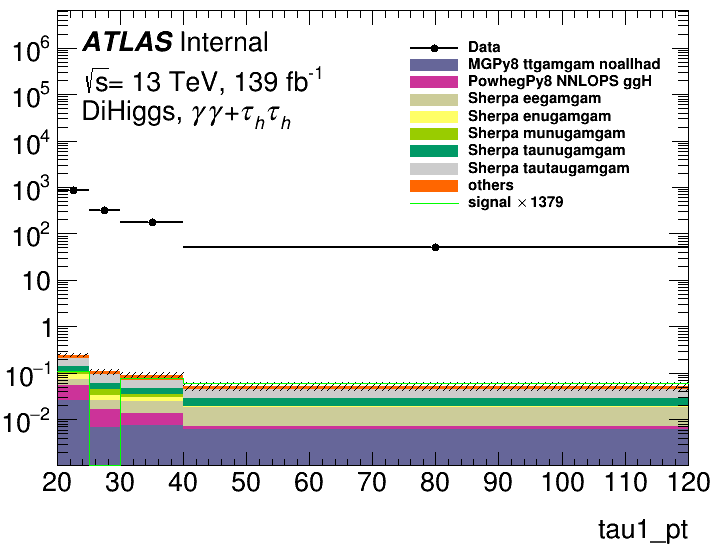
\includegraphics[width=0.45\textwidth]{figures/yy2tau/tau1_pt_CRfail_2taus_invertGam1_1p.png}
	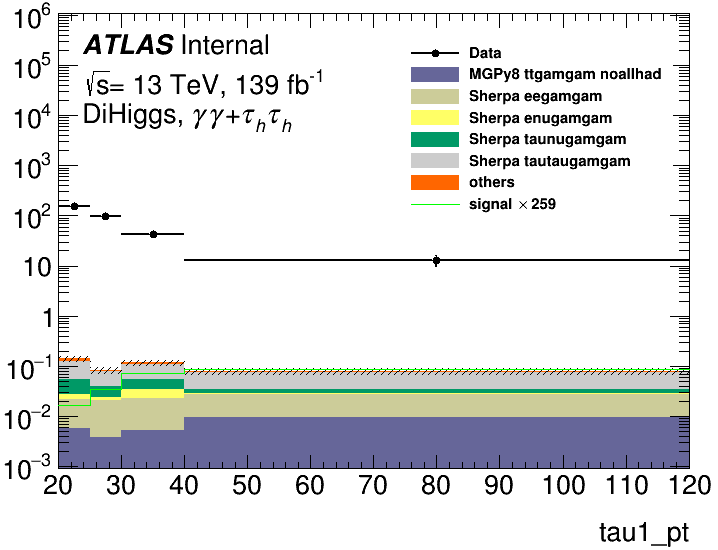
\includegraphics[width=0.45\textwidth]{figures/yy2tau/tau1_pt_CRpass_2taus_invertGam1_1p.png}
	\\
	\centering
	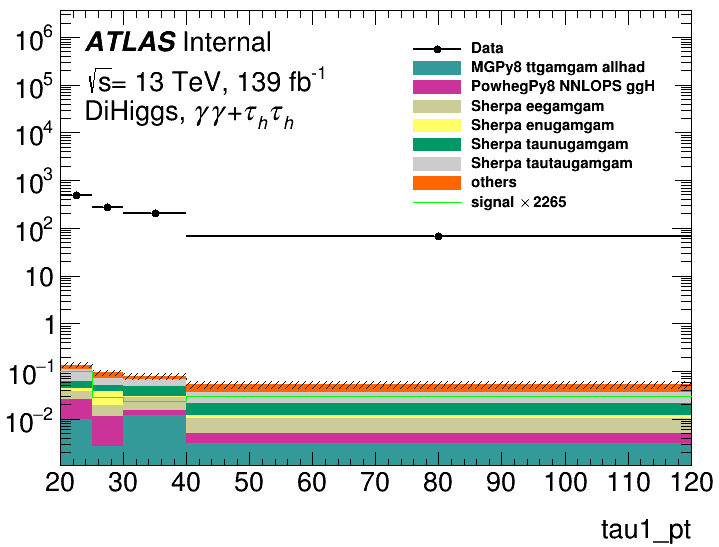
\includegraphics[width=0.45\textwidth]{figures/yy2tau/tau1_pt_CRfail_2taus_invertGam1_3p.png}
	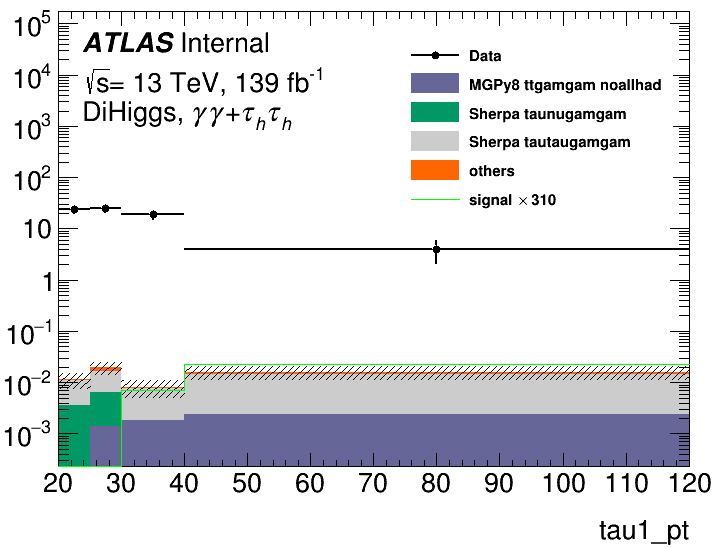
\includegraphics[width=0.45\textwidth]{figures/yy2tau/tau1_pt_CRpass_2taus_invertGam1_3p.png}\\
	\caption{\label{fig:yy2tau:FCRs} $p_{T}$ distributions in $FCR$ for 1-prong (top) and 3-prong (bottom) subleading \tauh candidate failing (left) / passing (right) loose tau-ID.}
\end{figure}

\begin{figure}
	\begin{center}
	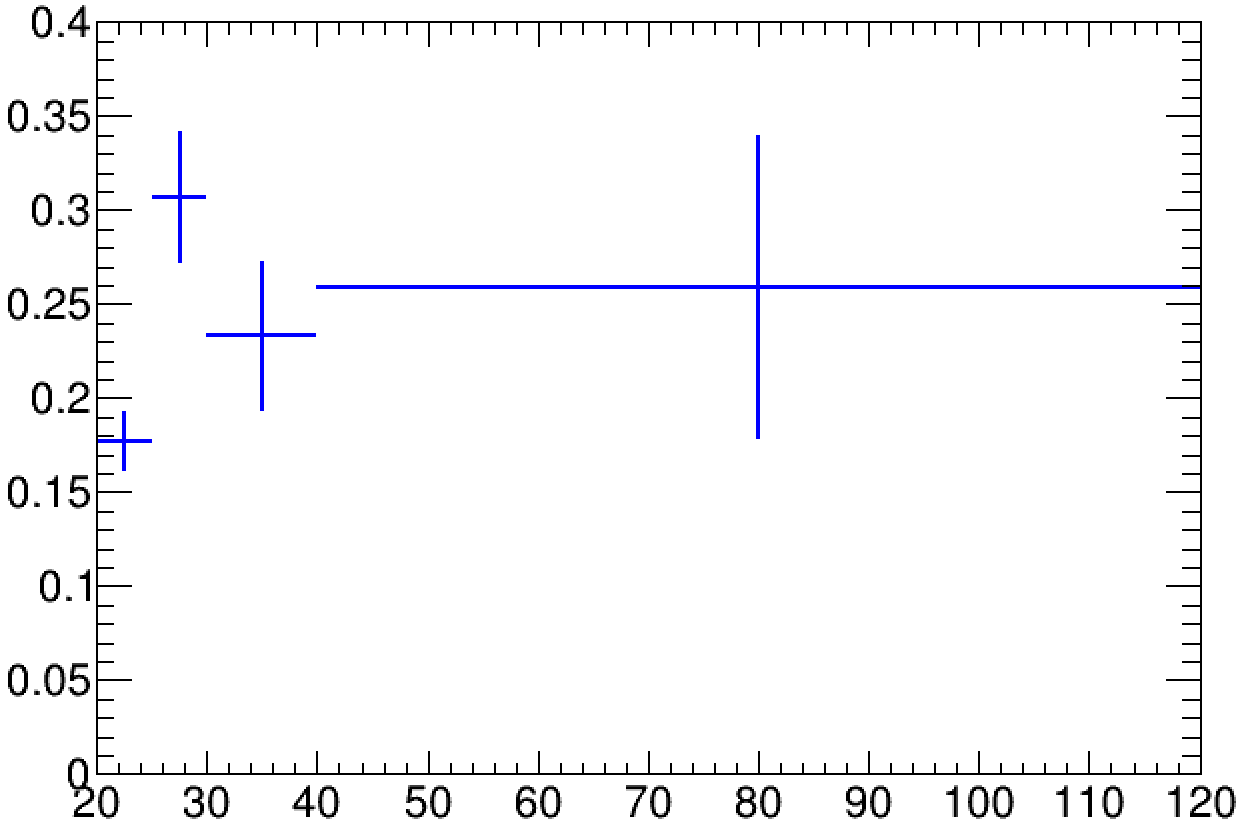
\includegraphics[width=0.45\textwidth]{figures/yy2tau/FF_1p.png}
	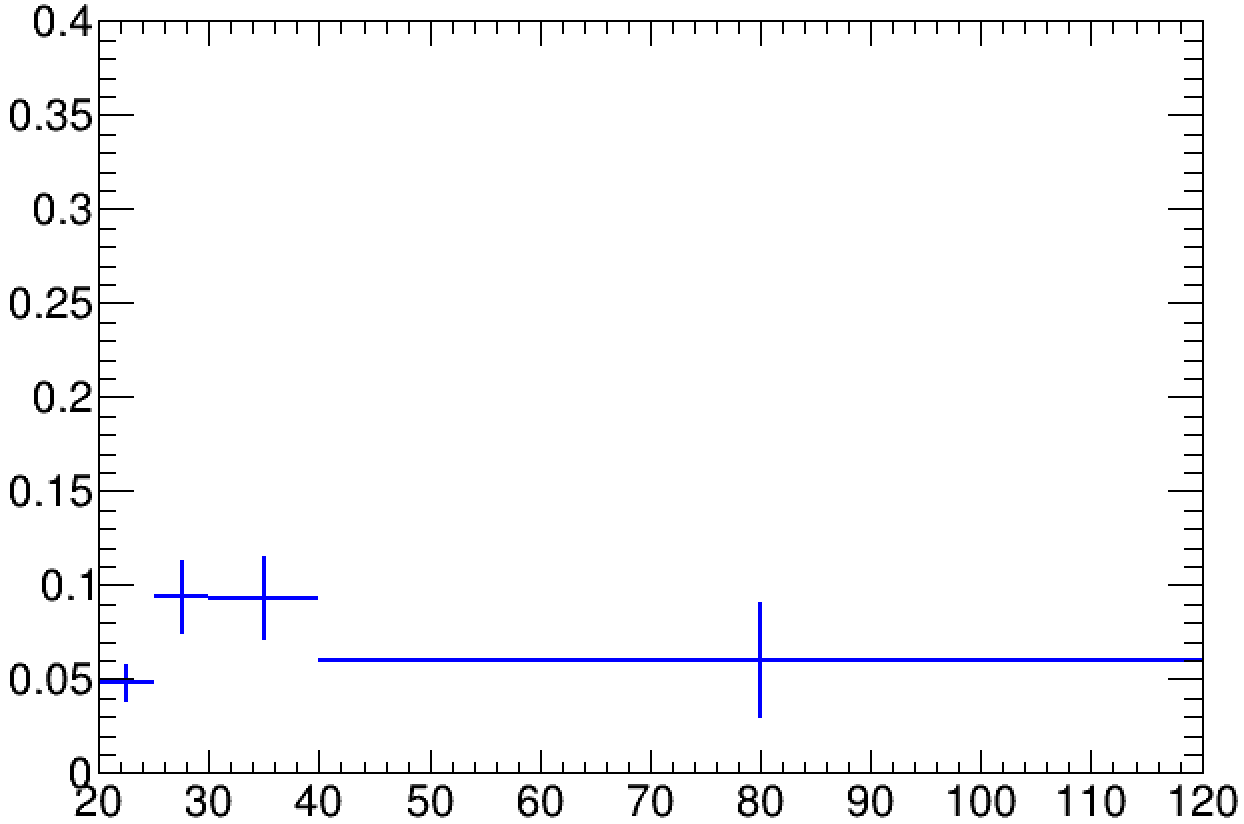
\includegraphics[width=0.45\textwidth]{figures/yy2tau/FF_3p.png}
	\caption{\label{fig:yy2tau:FFs} Fake factors depend on subleading \tauh $p_{T}$ for 1-prong (left) and 3-prong (right) \tauh. Error bars show statisticaly only uncertainty.}
	\end{center}
\end{figure}

\begin{figure}
	\centering
	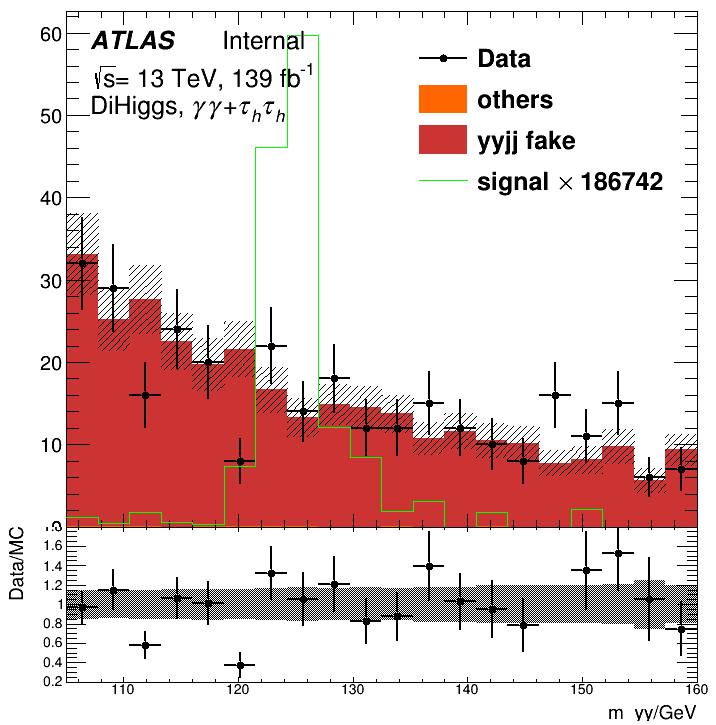
\includegraphics[width=0.45\textwidth]{figures/yy2tau/m_yy_Closure_CR_2taus_invertGam1_1p.png}
	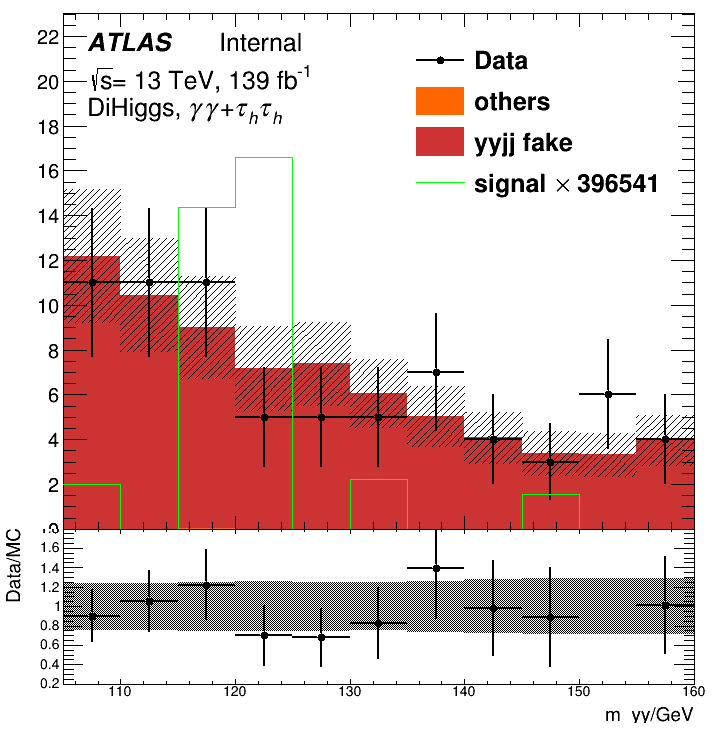
\includegraphics[width=0.45\textwidth]{figures/yy2tau/m_yy_Closure_CR_2taus_invertGam1_3p.png}\\
	\centering
	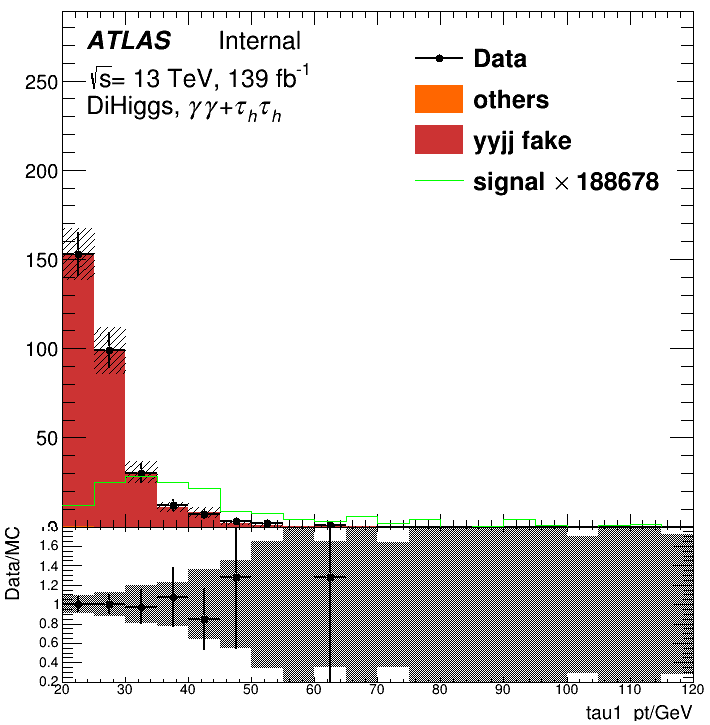
\includegraphics[width=0.45\textwidth]{figures/yy2tau/tau1_pt_Closure_CR_2taus_invertGam1_1p.png}
	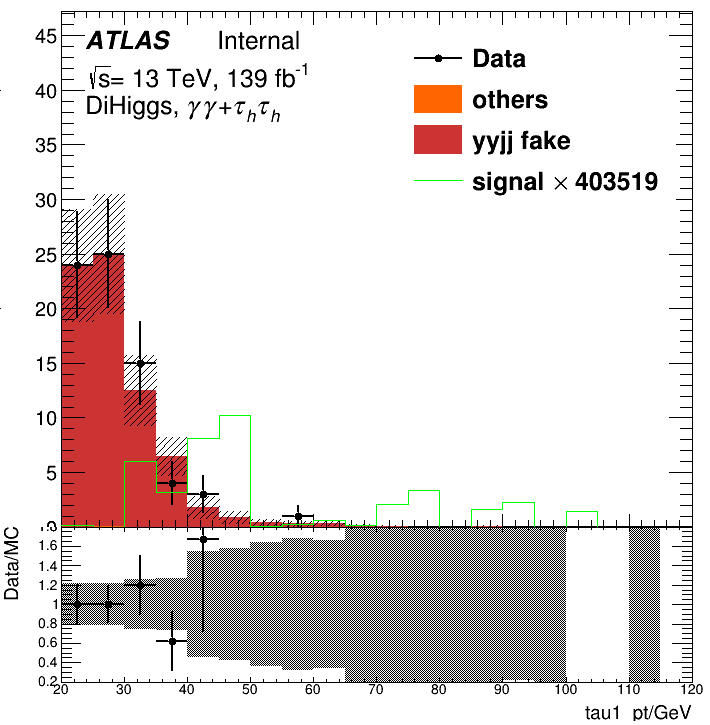
\includegraphics[width=0.45\textwidth]{figures/yy2tau/tau1_pt_Closure_CR_2taus_invertGam1_3p.png}\\
	\caption{\label{fig:yy2tau:Closure} Closure test performed with regard to \myy (upper) and ${p_{T}}_{\tau_{1}}$ (bottom) for 1-prong (left) and 3-prong (right) \tauh in. Event numbers of pass-ID region of FCR are estimated by applying fake factors back to event numbers of fail-ID region of FCR.}
\end{figure}

\begin{figure}
	\centering
	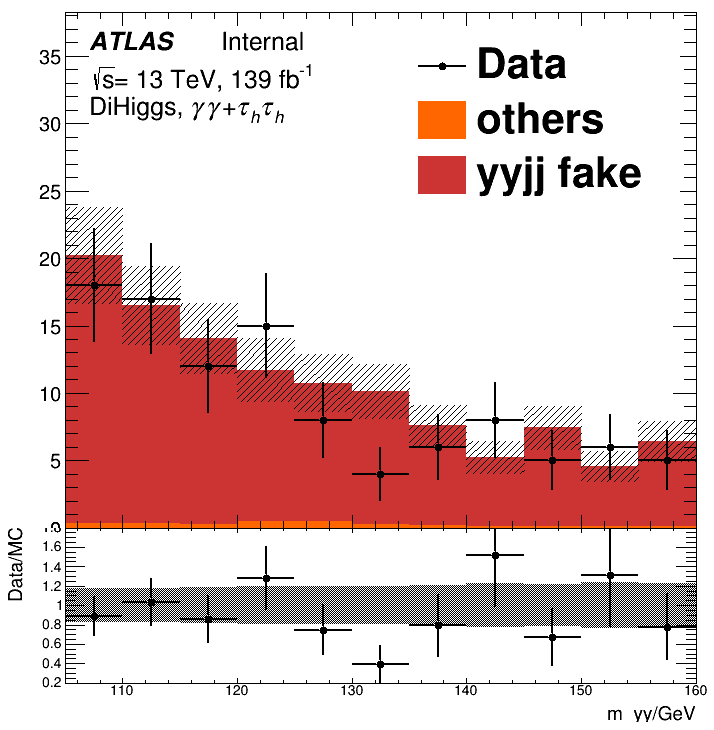
\includegraphics[width=0.45\textwidth]{figures/yy2tau/m_yy_VR_2taus_invertGam1.png}
	\caption{\label{fig:yy2tau:VRs} \myy distribution in the validatoin region}
\end{figure}

\subsubsection{MVA method}

BDT is trained to discriminate between the \yytwotau signal and major backgrounds including \yyjet (normalized to fake factor estimation), $ZH$, \Vyy ($\tau\tau\gamma\gamma$, $\tau\nu_{\tau}\gamma\gamma$). Kinematic variables used in BDT training can be categorized as follows:

Properties of the Higgs boson: the visible mass and transverse momentum of the di-$\tau$ system, ${m^{vis}_{\tau\tau}}$ ,${p_{T}}^{vis}_{\tau\tau}$, the transverse momentum and pseudorapidity of the di-$\gamma$ system, ${p_{T}}_{\gamma\gamma}$, $\eta_{\gamma\gamma}$.

Properties of resonnant di-$\tau$ and di-$\gamma$ decays: the angular distances $\Delta R_{\tau\tau}$ and $\Delta R_{\gamma\gamma}$

Visible transverse momentum of leading \tauh candidate ${p_{T}}_{\tau_{0}}$, missing transverse momentum $E^{miss}_{T}$ and scalar sum of $E_{T}$

The most important variables in the training are $\Delta R_{\gamma\gamma}$ and ${p_{T}}_{\gamma\gamma}$. The resulting BDT score distribution is shown in Fig.\ref{fig:yy2tau:BDT} for event pass the preselection and show the ability of the BDT to separate the signal process from background processes. The BDT score is used as observale in the final fit.

2-folds cross validation...

\begin{figure}
	\centering
	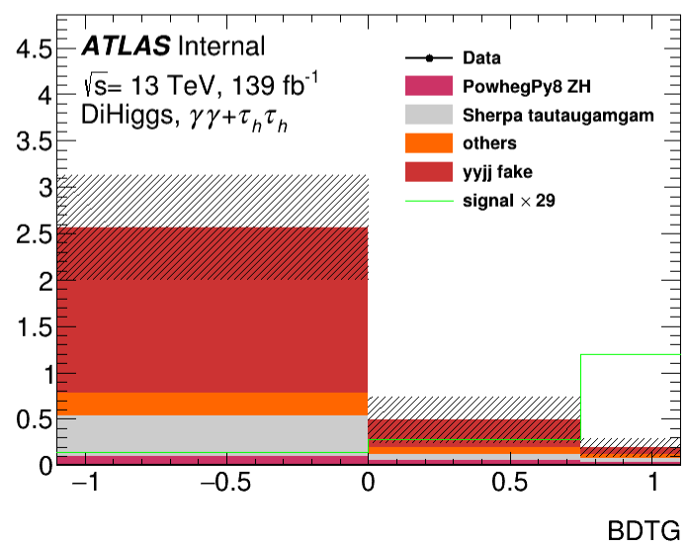
\includegraphics[width=0.45\textwidth]{figures/yy2tau/BDT.png}
	\caption{\label{fig:yy2tau:BDT} $BDT_{score}$ distribution after the preselection}
\end{figure}

\subsubsection{Results}